\begin{figure*}[t]
\centering
\begin{minipage}{.49\textwidth}
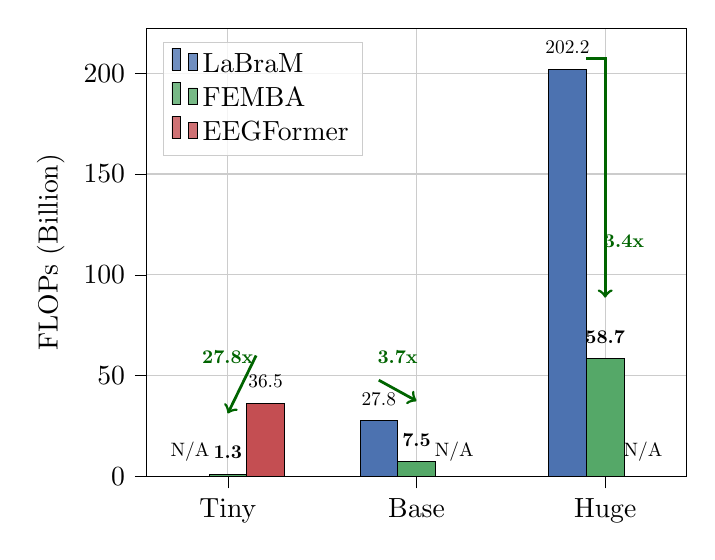
\begin{tikzpicture}

\definecolor{darkgreen}{RGB}{0,100,0}
\definecolor{gray}{RGB}{128,128,128}
\definecolor{indianred1967882}{RGB}{196,78,82}
\definecolor{lightgray204}{RGB}{204,204,204}
\definecolor{mediumseagreen85168104}{RGB}{85,168,104}
\definecolor{steelblue76114176}{RGB}{76,114,176}

\begin{axis}[
legend cell align={left},
legend style={
  fill opacity=0.8,
  draw opacity=1,
  text opacity=1,
  at={(0.03,0.97)},
  anchor=north west,
  draw=lightgray204
},
tick align=outside,
tick pos=left,
x grid style={black!20},
xmajorgrids,
xlabel near ticks,
xmin=-0.43, xmax=2.43,
xtick style={color=black},
xtick={0,1,2},
xticklabels={Tiny,Base,Huge},
y grid style={black!20},
ylabel={FLOPs (Billion)},
ymajorgrids,
ymin=0, ymax=222.31,
ytick style={color=black}
]
\draw[draw=black,fill=steelblue76114176,very thin] (axis cs:-0.3,0) rectangle (axis cs:-0.1,0);
\addlegendimage{ybar,ybar legend,draw=black,fill=steelblue76114176,very thin}
\addlegendentry{LaBraM}

\draw[draw=black,fill=steelblue76114176,very thin] (axis cs:0.7,0) rectangle (axis cs:0.9,27.8);
\draw[draw=black,fill=steelblue76114176,very thin] (axis cs:1.7,0) rectangle (axis cs:1.9,202.2);
\draw[draw=black,fill=mediumseagreen85168104,very thin] (axis cs:-0.1,0) rectangle (axis cs:0.1,1.3);
\addlegendimage{ybar,ybar legend,draw=black,fill=mediumseagreen85168104,very thin}
\addlegendentry{FEMBA}

\draw[draw=black,fill=mediumseagreen85168104,very thin] (axis cs:0.9,0) rectangle (axis cs:1.1,7.5);
\draw[draw=black,fill=mediumseagreen85168104,very thin] (axis cs:1.9,0) rectangle (axis cs:2.1,58.7);
\draw[draw=black,fill=indianred1967882,very thin] (axis cs:0.1,0) rectangle (axis cs:0.3,36.5);
\addlegendimage{ybar,ybar legend,draw=black,fill=indianred1967882,very thin}
\addlegendentry{EEGFormer}

\draw[draw=black,fill=indianred1967882,very thin] (axis cs:1.1,0) rectangle (axis cs:1.3,0);
\draw[draw=black,fill=indianred1967882,very thin] (axis cs:2.1,0) rectangle (axis cs:2.3,0);
\draw (axis cs:-0.2,0) ++(0pt,3pt) node[
  scale=0.7,
  anchor=south,
  text=black,
  rotate=0.0
]{N/A};
\draw (axis cs:0.8,27.8) ++(0pt,3pt) node[
  scale=0.7,
  anchor=south,
  text=black,
  rotate=0.0
]{27.8};
\draw (axis cs:1.8,202.2) ++(0pt,3pt) node[
  scale=0.7,
  anchor=south,
  text=black,
  rotate=0.0
]{202.2};
\draw (axis cs:0,1.3) ++(0pt,3pt) node[
  scale=0.7,
  anchor=south,
  text=black,
  rotate=0.0
]{\bfseries 1.3};
\draw (axis cs:1,7.5) ++(0pt,3pt) node[
  scale=0.7,
  anchor=south,
  text=black,
  rotate=0.0
]{\bfseries 7.5};
\draw (axis cs:2,58.7) ++(0pt,3pt) node[
  scale=0.7,
  anchor=south,
  text=black,
  rotate=0.0
]{\bfseries 58.7};
\draw (axis cs:0.2,36.5) ++(0pt,3pt) node[
  scale=0.7,
  anchor=south,
  text=black,
  rotate=0.0
]{36.5};
\draw (axis cs:1.2,0) ++(0pt,3pt) node[
  scale=0.7,
  anchor=south,
  text=black,
  rotate=0.0
]{N/A};
\draw (axis cs:2.2,0) ++(0pt,3pt) node[
  scale=0.7,
  anchor=south,
  text=black,
  rotate=0.0
]{N/A};
\draw[<-, draw=darkgreen, line width=1pt] (axis cs:0,31.3) -- (axis cs:0.15,60);

\draw (axis cs:0,59.3) node[
  scale=0.7,
  text=darkgreen,
  rotate=0.0
]{\bfseries 27.8x};
\draw[<-,draw=darkgreen, line width=1pt] (axis cs:1,37.5) -- (axis cs:0.8,47.8);
\draw (axis cs:0.9,59.3) node[
  scale=0.7,
  text=darkgreen,
  rotate=0.0
]{\bfseries 3.7x};
\draw[-,draw=darkgreen,line width=1pt] (axis cs:2.01,207.2) -- (axis cs:1.9,207.2);
\draw[<-,draw=darkgreen,line width=1pt] (axis cs:2,88.7) -- (axis cs:2,207.7);
\draw (axis cs:2.1,116.7) node[
  scale=0.7,
  text=darkgreen,
  rotate=0.0
]{\bfseries 3.4x};
\end{axis}

\end{tikzpicture}
\end{minipage}
\begin{minipage}{.5\textwidth}

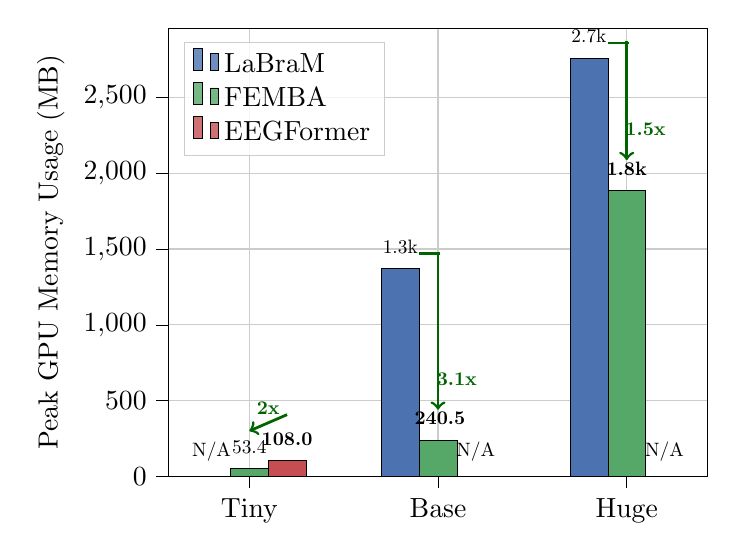
\begin{tikzpicture}

\definecolor{darkgreen}{RGB}{0,100,0}
\definecolor{gray}{RGB}{128,128,128}
\definecolor{indianred1967882}{RGB}{196,78,82}
\definecolor{lightgray204}{RGB}{204,204,204}
\definecolor{mediumseagreen85168104}{RGB}{85,168,104}
\definecolor{steelblue76114176}{RGB}{76,114,176}

\begin{axis}[
legend cell align={left},
legend style={
  fill opacity=0.8,
  draw opacity=1,
  text opacity=1,
  at={(0.03,0.97)},
  anchor=north west,
  draw=lightgray204
},
tick align=outside,
tick pos=left,
x grid style={black!20},
xmajorgrids,
xlabel near ticks,
xmin=-0.43, xmax=2.43,
xtick style={color=black},
xtick={0,1,2},
xticklabels={Tiny,Base,Huge},
y grid style={black!20},
ylabel={Peak GPU Memory Usage (MB)},
ymajorgrids,
ymin=0, ymax=2955.32,
ytick style={color=black}
]
\draw[draw=black,fill=steelblue76114176,very thin] (axis cs:-0.3,0) rectangle (axis cs:-0.1,0);
\addlegendimage{ybar,ybar legend,draw=black,fill=steelblue76114176,very thin}
\addlegendentry{LaBraM}

\draw[draw=black,fill=steelblue76114176,very thin] (axis cs:0.7,0) rectangle (axis cs:0.9,1371.9);
\draw[draw=black,fill=steelblue76114176,very thin] (axis cs:1.7,0) rectangle (axis cs:1.9,2758.4);
\draw[draw=black,fill=mediumseagreen85168104,very thin] (axis cs:-0.1,0) rectangle (axis cs:0.1,53.4);
\addlegendimage{ybar,ybar legend,draw=black,fill=mediumseagreen85168104,very thin}
\addlegendentry{FEMBA}

\draw[draw=black,fill=mediumseagreen85168104,very thin] (axis cs:0.9,0) rectangle (axis cs:1.1,240.5);
\draw[draw=black,fill=mediumseagreen85168104,very thin] (axis cs:1.9,0) rectangle (axis cs:2.1,1886.2);
\draw[draw=black,fill=indianred1967882,very thin] (axis cs:0.1,0) rectangle (axis cs:0.3,108);
\addlegendimage{ybar,ybar legend,draw=black,fill=indianred1967882,very thin}
\addlegendentry{EEGFormer}

\draw[draw=black,fill=indianred1967882,very thin] (axis cs:1.1,0) rectangle (axis cs:1.3,0);
\draw[draw=black,fill=indianred1967882,very thin] (axis cs:2.1,0) rectangle (axis cs:2.3,0);
\draw (axis cs:-0.2,0) ++(0pt,3pt) node[
  scale=0.7,
  anchor=south,
  text=black,
  rotate=0.0
]{N/A};
\draw (axis cs:0.8,1371.9) ++(0pt,3pt) node[
  scale=0.7,
  anchor=south,
  text=black,
  rotate=0.0
]{1.3k};
\draw (axis cs:1.8,2758.4) ++(0pt,3pt) node[
  scale=0.7,
  anchor=south,
  text=black,
  rotate=0.0
]{2.7k};
\draw (axis cs:0,53.4) ++(0pt,3pt) node[
  scale=0.7,
  anchor=south,
  text=black,
  rotate=0.0
]{53.4};
\draw (axis cs:1.01,240.5) ++(0pt,3pt) node[
  scale=0.7,
  anchor=south,
  text=black,
  rotate=0.0
]{\bfseries 240.5};
\draw (axis cs:2,1886.2) ++(0pt,3pt) node[
  scale=0.7,
  anchor=south,
  text=black,
  rotate=0.0
]{\bfseries 1.8k};
\draw (axis cs:0.2,108) ++(0pt,3pt) node[
  scale=0.7,
  anchor=south,
  text=black,
  rotate=0.0
]{\bfseries 108.0};
\draw (axis cs:1.2,0) ++(0pt,3pt) node[
  scale=0.7,
  anchor=south,
  text=black,
  rotate=0.0
]{N/A};
\draw (axis cs:2.2,0) ++(0pt,3pt) node[
  scale=0.7,
  anchor=south,
  text=black,
  rotate=0.0
]{N/A};
\draw[<-,draw=darkgreen, line width=1pt] (axis cs:0,300.4) -- (axis cs:0.2,408);
\draw (axis cs:0.1,453.4) node[
  scale=0.7,
  text=darkgreen,
  rotate=0.0
]{\bfseries 2x};
\draw[-,draw=darkgreen, line width=1pt] (axis cs:1.01,1471.9) -- (axis cs:0.9,1471.9);
\draw[<-,draw=darkgreen,line width=1pt] (axis cs:1,440.5) -- (axis cs:1,1481.9);
\draw (axis cs:1.1,640.5) node[
  scale=0.7,
  text=darkgreen,
  rotate=0.0
]{\bfseries 3.1x};
\draw[-,draw=darkgreen, line width=1pt] (axis cs:2.01,2858.4) -- (axis cs:1.9,2858.4);
\draw[<-,draw=darkgreen, line width=1pt] (axis cs:2,2086.2) -- (axis cs:2,2868.4);
\draw (axis cs:2.1,2286.2) node[
  scale=0.7,
  text=darkgreen,
  rotate=0.0
]{\bfseries 1.5x};
\end{axis}

\end{tikzpicture}

\end{minipage}
\caption{Comparison of LaBraM~\cite{jianglarge}, \textbf{FEMBA}, and EEGFormer~\cite{chen2024eegformer} in terms of computational inference (left) and memory usage (in megabytes, MB) (right)}\label{fig:comparison_inference_gpu}

\end{figure*}
